\section{Dipendenza}
È lo stato di una cosa che è influenzato o determinato da qualcos'altro.

Ci sono 2 tipologie di cambiamenti:
\begin{itemize}
\item interno: cambiamenti di implementazione, quindi il cambiamento del corpo di una funzione;
\item estero: è un cambiamento dell’interfaccia, delle firma della funzione.
\end{itemize}

La dipendenza diventa quindi la probabilità che se una componente cambia internamento o esternamente anche le componenti che dipendono da essa cambiano. Tanto più il grado di dipendenza è alto, tanto più alta è la probabilità. Quindi la dipendenza e la probabilità è direttamente proporzionale.

\subsection{Accoppiamento}
\begin{itemize}
\item \textbf{tightly coupled}: accoppiamento forte, forte probabilità che le componenti cambino;
\item \textbf{loosely coupled}: accoppiamento lasco, è quello da preferire, bassa probabilità che le componenti cambino.
\end{itemize}

\textbf{test di unità}: è un test automatico che verifica le proprietà della componente presa singolarmente, senza le dipendenze esterne.

Per ogni componente dovremmo avere associato un test di unità. Per esempio un test di unità potrebbe dare in input uno 0 oppure numeri negativi, numeri molto grandi, ecc. Quindi questi test verificano la pre e la post di ogni metodo.

Modificando una componente, posso verificare che quest’ultimo sia ancora integro.

\subsection{Dipendenza in OOP}
Nella programmazione procedurale la dipendenza si misura tra procedure.

Mentre nella programmazione funzionale la componente principale è la funzione o il modulo.

Nella OOP la componente principale è la classe. Possiamo definire 5 tipi di dipendenza. Misuriamo quante righe di codice sono condivise tra 2 classi e per quanto tempo della loro vita (scope) sono in dipendeza.

\subsubsection{Dipendenza(Relazione)}
È molto lasca perché è limitata nel tempo in cui viene utilizzata e nelle righe di codice che vengono condivise tra 2 classi.

Una classe C1 dipende da una classe C2 se si verifica almeno una delle seguenti:
\begin{itemize}
\item deriva da C2;
\item invoca operazioni di C2 (anche solo un costruttore);
\item un suo attributo è di tipo C2;
\item un parametro di una sua operazione è di tipo C2;
\item accede ai campi di C2.
\end{itemize}

Una classe dipende da un interface se:
\begin{itemize}
\item realizza tale interface (si dice che fornisce quell’interface);
\item richiede tale interface (relazione uses).

\end{itemize}

\subsubsection{Associazione}
\begin{figure}[H]
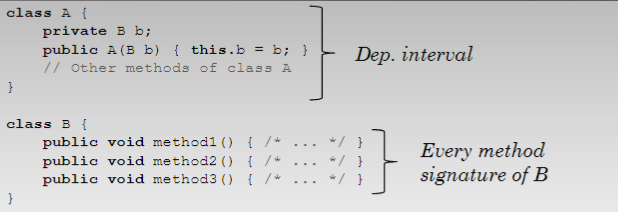
\includegraphics[scale=0.8]{images/asssociazione}
\caption{\textit{Esempio Associazione} \label{fig:ered5}}
\end{figure}

Qual’è lo scopo di dipendenza tra A e B? Siccome stò utilizzando dentro A un oggetto di tipo B, e costruisco A con quel oggetto, l’istanza di B dovrà sempre esistere, quindi ogni metodo di A può usare un istanza di B. Quindi lo scopo è tutta la classe A.

Le firme di tutti i metodi di B possono essere utilizzate in A, quindi è codice condiviso.

Una classe A utilizza una classe B se un oggetto della classe A è in grado di inviare dei messaggi ad un oggetto di classe B oppure se un oggetto di classe A può creare, ricevere o restituire oggetti di classe B.

\subsection{Aggregazione e composizione}
Sono un caso speciale dell’associazione perché un tipo possiede completamente l’altro.

Per esempio le celle di una scacchiera. Perchè sono possedute dalla scacchiera. Una cella non ha senso di esistere al di fuori della scacchiera.

\textbf{L'aggregazione} è una relazione puramente logica. I due oggetti esistono anche se sparisce la relazione. Nell'aggregazione invece tu usi un oggetto come attributo di una nuova classe lo stesso, ma qui non lo vai anche a creare, bensì lo ricevi dall'esterno, ciò significa che l'oggetto aggregante esiste a priori e quindi il ciclo di vita dell'oggetto aggregante è > del ciclo di vita dell'oggetto aggregato.

\textbf{La composizione}, invece, è una relazione più forte. L'oggetto contenuto non può esistere senza il contenitore. Nella composizione tu utilizzi un oggetto come attributo di una nuova classe, ciò comporta che il ciclo di vita dell'oggetto componente ( ex string ) è lo <= del ciclo di vita dell'oggetto composto.

Nella pratica la composizione la tieni quando hai dichiari una reference a string e fai anche la new, l'aggregazione invece quando dichiari solo la reference a string e poi tipo nel costruttore passi un riferimento ad una stringa che è stata creata precedentemente.
\subsubsection{SLOC}

\textbf{SLOC}: source line of code

Quando posso calcolare le linee di codice condivise tra 2 componenti posso formalizzare attraverso una formula matematica, il grado di dipendenza tra i 2 componenti:
\begin{figure}[H]
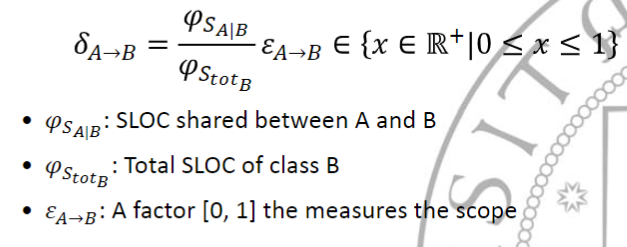
\includegraphics[scale=0.8]{images/SLOC}
\caption{\textit{Definizione di SLOC} \label{fig:sloc}}
\end{figure}
numero linee di codice condivise tra a e b DIVISO il numero di linee complessive di B. Quando ho una dipendenza di tipo Ereditarietà questo limite tende a 1.

Non basta il tipo di dipendenza perché c’è anche lo \textbf{scope}, ovvero il fattore temporale, calcolato in epsilon e cambia a seconda della tipologia di dipendenza. Serve a dar un ordine di importanza alla dipendeze. Per esempio \textbf{l’ereditarietà} ha un epsilon grande in modo da portare l’equazione a 100\%. Più grande è epsion più alta e  la dipendenza. Quindi bisogna scegliere un epsion piccolo.

\textbf{Osservazione}: \textit{Se implemento un’interfaccia oppure se estendo una classe che ha solamente metodi virtuali puri, che tipo di dipendeza c’è?}

L’interfaccia essendo solamente un contratto non è una classe quindi non c’è dipendenza.
